% ============================================================
% SUPPLEMENT 3: Toy-to-Real Bridge
% The Geometry of SAE Artifacts Research Program
% Bridging Phase 2 (Toy-Model Validation) to Phase 3 (Seed Stability)
% March 2026
% ============================================================
\documentclass[11pt,a4paper]{article}

\usepackage[utf8]{inputenc}
\usepackage[T1]{fontenc}
\usepackage{times}
\usepackage{amsmath,amssymb,amsfonts,amsthm}
\usepackage{graphicx}
\usepackage{booktabs}
\usepackage{hyperref}
\usepackage[margin=1in]{geometry}
\usepackage{enumitem}
\usepackage{caption}
\usepackage{subcaption}
\usepackage{natbib}
\usepackage{xcolor}
\usepackage{microtype}
\usepackage{float}
\usepackage{fancyhdr}
\usepackage{multirow}
\usepackage{array}
\usepackage{longtable}
\usepackage{tcolorbox}
\usepackage{colortbl}

\graphicspath{{../}}

\hypersetup{colorlinks=true,linkcolor=blue!60!black,citecolor=blue!60!black,urlcolor=blue!60!black}

%% Coloured boxes matching Phase 2 style
\newtcolorbox{keyinsight}{colback=blue!5!white,colframe=blue!50!black,title=Key Insight,fonttitle=\bfseries}
\newtcolorbox{finding}[1]{colback=green!5!white,colframe=green!50!black,title=#1,fonttitle=\bfseries}
\newtcolorbox{revealed}{colback=red!5!white,colframe=red!50!black,title=Unexpected Finding,fonttitle=\bfseries}
\newtcolorbox{prereg}{colback=yellow!5!white,colframe=orange!60!black,title=Pre-Registration (written before running),fonttitle=\bfseries}
\newtcolorbox{gatebox}[1]{colback=orange!5!white,colframe=orange!70!black,title=Gate Condition #1,fonttitle=\bfseries\large}
\newtcolorbox{limitation}{colback=gray!5!white,colframe=gray!40!black,title=Limitation Addressed,fonttitle=\bfseries}

\newtheorem{remark}{Remark}
\newtheorem{proposition}{Proposition}

\setlength{\parskip}{0.4em}
\setlength{\parindent}{1.5em}

\pagestyle{fancy}
\fancyhf{}
\rhead{\small\textit{Supplement 3: Toy-to-Real Bridge}}
\lhead{\small\textit{Geometry of SAE Artifacts --- March 2026}}
\cfoot{\thepage}

%% Shorthand commands
\newcommand{\cosED}{\cos(E_i, D_i)}
\newcommand{\nneg}{n_{\mathrm{neg}}}
\newcommand{\mcos}{\bar{c}_{\min}}
\newcommand{\lambdaL}{\lambda_{\mathrm{L1}}}
\newcommand{\Ef}{E_f}
\newcommand{\Df}{D_f}
\newcommand{\jenc}{j_{\mathrm{enc}}}
\newcommand{\jdec}{j_{\mathrm{dec}}}
\DeclareMathOperator*{\argmax}{arg\,max}

% ============================================================
\title{\Large\bfseries Supplement 3 Report: Toy-to-Real Bridge\\[0.5em]
\large The Geometry of SAE Artifacts Research Program\\[0.3em]
\normalsize Closing Gaps Between Phase~2 (G2-YES) and Phase~3 (Seed Stability)}
\author{\textit{Working Report --- March 2026}\\[0.3em]
\small Three sub-experiments: S3A (bisector test, real GPT-2 L8 SAE),
S3B (expansion ratio sweep), S3C (seed distribution, 100 seeds)}
\date{}

% ============================================================
\begin{document}
\maketitle
\thispagestyle{fancy}

\begin{abstract}
\noindent Phase~2 established gate G2-YES: anti-aligned encoder/decoder feature pairs
($\cosED < 0$) arise from a fundamental geometric property of the SAE bottleneck
optimisation, not from any particular sparsity mechanism.  Three limitations remained
before the GPU-intensive Phase~3 (Seed Stability) could be launched:
\textbf{Limitation~4}---the toy-model ``inhibitory bisector'' (hedge) mechanism was
never tested on a real SAE;
\textbf{Limitation~5}---the expansion-ratio sweep (Experiment~2D) was never run; and
\textbf{Limitation~2}---seed dependence was not quantified statistically.

This supplement addresses all three through pre-registered sub-experiments.
\textbf{S3A} applies a bisector test to the Bloom GPT-2 Layer-8 SAE
($d_{\mathrm{model}}{=}768$, $d_{\mathrm{SAE}}{=}24576$) and finds the hedge structure
confirmed in 3 of 4 tested anti-aligned features, including an unexpected
\emph{Hedge Family}: all four features target the same polysemantic parent cluster
$\{$F17487, F21174, F16152$\}$.
\textbf{S3B} sweeps the SAE expansion ratio from 1$\times$ to 32$\times$ on a 10D toy
model and discovers a sharp phase transition at ${\approx}5$--$6\times$: below this
threshold anti-alignment is essentially absent; above it the phenomenon becomes nearly
inevitable ($P{\to}1.00$).  At 32$\times$ (the expansion ratio of the Bloom GPT-2 SAE) the
toy model produces $\nneg{=}82.95{\pm}4.96$ out of 320 features.
\textbf{S3C} runs 100 seeds at 3$\times$ expansion and finds $P(\nneg{\ge}1){=}0.13$
for both $\lambda{=}0$ and $\lambda{=}5\!\times\!10^{-3}$, confirming that lambda has
zero effect on the probability.

All three pre-registered predictions were \emph{wrong in direction}, which led to a
deeper and more satisfying theory: anti-alignment requires two conditions---sufficient
expansion ratio ($>{5}\times$) and polysemantic superposition pressure.
Phase 3 is revised accordingly: $H_{\mathrm{UNSTABLE}}$ is unlikely, and the central
question shifts to whether the specific Hedge Family is stable across seeds.
\end{abstract}

\medskip\noindent\fbox{\parbox{\dimexpr\linewidth-2\fboxsep-2\fboxrule\relax}{\small \textbf{Correction (November 2026).} An earlier version claimed a close quantitative match between the toy model at $32\times$ ($\nneg = 82.95$) and ``${\approx}86$'' anti-aligned features in the real GPT-2 Layer-8 SAE. The real Layer-8 SAE has 4 features with $\cosED<0$; 86 was an artefact of a truncated table (E1). The fractions (25.9\% of a 320-feature toy dictionary vs.\ 0.016\% of 24{,}576) are not comparable. The match claim has been removed, and conclusions about Phase~3 power that relied on it are now stated for the toy model only. See \texttt{docs/ERRATA.md} in the repository for details.}}

\vspace{0.5em}\hrule\vspace{0.5em}
\tableofcontents
\newpage

% ============================================================
\section{Objective and Gap Analysis}
\label{sec:objective}

\subsection{Research Program Context}

The ``Geometry of SAE Artifacts'' program investigates why a non-trivial fraction of
learned SAE features have encoder directions $E_i$ and decoder directions $D_i$ that
are \emph{anti-aligned}, i.e.\ $\cosED < 0$.  Phase~2 established through toy-model
experiments that this is a geometric property of the bottleneck optimisation, not an
artifact of the L1 penalty or any specific sparsity mechanism, yielding gate decision
\textbf{G2-YES}.

Phase~3 is the next planned phase: a seed-stability study using GPU resources to test
whether anti-aligned features in a real SAE are reproducible across training seeds.
Phase~3 has three hypotheses:
\begin{description}[leftmargin=1em,noitemsep]
  \item[$H_{\mathrm{UNSTABLE}}$] Anti-aligned features are artefacts of a specific
    random seed; different seeds produce fewer than two such features.
  \item[$H_{\mathrm{STABLE}}$] The \emph{same} specific features are anti-aligned
    across all seeds.
  \item[$H_{\mathrm{STAT\_STABLE}}$] The statistical \emph{count} of anti-aligned
    features is consistent across seeds, but the specific features differ.
\end{description}

\subsection{Three Gaps Addressed by This Supplement}

\begin{limitation}
\textbf{Limitation~4 (from Phase~2 limitations list):} The ``inhibitory bisector'' or
hedge mechanism proposed in Phase~2 was demonstrated only in toy models.  It has
\emph{never been tested on a real trained SAE} from the empirical corpus (GPT-2,
Gemma, Llama).  Phase~3 uses this as the primary mechanistic lens; a failed bisector
test would require adding activation-frequency analysis first.
\end{limitation}

\begin{limitation}
\textbf{Limitation~5 (from Phase~2 limitations list):} The expansion-ratio sweep
(labelled Experiment~2D in the Phase~2 plan) was never executed.  Phase~2 used a
fixed $d_{\mathrm{model}}{=}10$, $d_{\mathrm{SAE}}{=}20$ (2$\times$ expansion),
while the real GPT-2 Bloom SAE operates at 32$\times$.  Without this sweep we cannot
extrapolate Phase~2 toy-model findings to real-world SAE widths.
\end{limitation}

\begin{limitation}
\textbf{Limitation~2 (from Phase~2 limitations list):} Phase~2 used only three random
seeds per configuration.  The probability $P(\nneg \ge 1)$ under a fixed expansion
and $\lambda$ value was never estimated with enough statistical power.
Phase~3 needs this estimate to justify its sample-size design.
\end{limitation}

\subsection{Supplement Structure}

Section~\ref{sec:prereg} states all pre-registered predictions.
Sections~\ref{sec:s3a}--\ref{sec:s3c} present each sub-experiment.
Section~\ref{sec:gate} evaluates the gate conditions for Phase~3.
Section~\ref{sec:discussion} discusses implications and what must be
revised in the Phase~3 protocol.

% ============================================================
\section{Pre-Registration}
\label{sec:prereg}

All predictions below were written in the research notebook \emph{before any data were
collected or scripts were run}.  Pre-registration prevents post-hoc rationalisation
and forces us to acknowledge surprises.

\begin{prereg}
\textbf{S3A (Bisector Test on Real SAE):}
\begin{itemize}[noitemsep]
  \item Feature F19139 (encoder norm ${\approx}0.727$, well above mean): hedge
    structure \textbf{PRESENT}.  Prediction: $\cos(\Df, D_{\jenc}) < 0$.
  \item Feature F18573 (encoder norm ${\approx}0.233$, well below mean): hedge
    structure \textbf{ABSENT}.  Prediction: feature is dead or lacks coherent
    geometric structure due to small encoder norm.
\end{itemize}

\textbf{S3B (Expansion Ratio Sweep):}
\begin{itemize}[noitemsep]
  \item Prediction: $\nneg$ \emph{decreases} as the expansion ratio increases.
    Rationale: more SAE features $\Rightarrow$ easier to represent each concept
    cleanly $\Rightarrow$ less need for inhibitory hedging.
\end{itemize}

\textbf{S3C (Seed Distribution):}
\begin{itemize}[noitemsep]
  \item Sub-prediction~1: $P(\nneg{\ge}1 \mid \lambda{=}5\times10^{-3}) >
    P(\nneg{\ge}1 \mid \lambda{=}0)$, because L1 regularisation organises the
    loss landscape and makes hedge solutions more accessible.
  \item Sub-prediction~2: $P(\nneg{\ge}1)$ lies in $[0.30,\,0.70]$ for both
    $\lambda$ values.
  \item Sub-prediction~3: The coefficient of variation of $\nneg$ (when $\nneg>0$)
    is small ($<0.5$), indicating limited seed-to-seed variability.
\end{itemize}
\end{prereg}

\textbf{Outcome summary (see Appendix~\ref{app:scorecard} for full scorecard):}
All three main predictions were wrong in direction.  The data reveal a richer
structure than anticipated: the key variable is expansion ratio, not $\lambda$.

% ============================================================
\section{S3A: Bisector Test on Real GPT-2 Layer-8 SAE}
\label{sec:s3a}

\subsection{Setup and Notation}

We loaded the Bloom GPT-2-small Layer-8 residual-stream SAE
(\texttt{gpt2-small-res-jb}, hook \texttt{blocks.8.hook\_resid\_pre})~\citep{bloom2024},
with $d_{\mathrm{model}}{=}768$ and $d_{\mathrm{SAE}}{=}24{,}576$ (32$\times$ expansion).
The empirical distribution of $\cos(\Ef, \Df)$ across all features has
$\mu{=}0.3683$, $\sigma{=}0.0785$.

The bisector-hedge mechanism predicts that an anti-aligned feature $f$ functions as
an ``inhibitory gate'' against a cluster of aligned features.  Specifically:
\begin{enumerate}[noitemsep]
  \item The encoder $\Ef$ points \emph{toward} the decoder directions of the aligned
    cluster, making $f$ fire when those features are active.
  \item The decoder $\Df$ points \emph{away} from those same directions, so whenever
    $f$ fires it \emph{subtracts} a component of the cluster from the reconstruction.
\end{enumerate}
We operationalise this with two quantities.  Let
$j^* = \jenc \equiv \argmax_j \cos(\Ef, D_j)$ be the aligned feature whose decoder
the encoder of $f$ most detects.  Then:
\begin{align}
  \cos(\Ef,\, D_{j^*}) &> 0 \quad \text{(encoder detects parent)}, \label{eq:enc}\\
  \cos(\Df,\, D_{j^*}) &< 0 \quad \text{(decoder opposes parent)}. \label{eq:dec}
\end{align}
Equation~\eqref{eq:dec} is the \textbf{bisector-hedge prediction}.
We define the \textbf{bisector score}
$s_f = \cos(\Ef, D_{j^*}) \cdot (-\cos(\Df, D_{j^*}))$;
a positive score indicates both conditions hold simultaneously.

We selected the four most anti-aligned features in the SAE by $\cos(\Ef, \Df)$:
F19139, F18573, F11969, and F20804.  Features F19139 and F18573 were the only two
features explicit in the pre-registration (Section~\ref{sec:prereg}).

\subsection{Results}

\begin{table}[H]
\centering
\caption{Bisector-hedge test results on the four most anti-aligned features of the
Bloom GPT-2 Layer-8 SAE.  Column ``$\sigma$-dev'' gives the number of standard
deviations below the population mean $\mu{=}0.3683$.  Column ``$j^*$'' is the
aligned feature whose decoder $\Ef$ most detects.
Bisector score $s_f > 0$ indicates confirmed hedge structure.}
\label{tab:bisector}
\begin{tabular}{@{}lcrrrccrr@{}}
\toprule
Feature & $\cos(\Ef,\Df)$ & $\sigma$-dev & $\|\Ef\|$ & $j^*$ &
  $\cos(\Ef, D_{j^*})$ & $\cos(\Df, D_{j^*})$ & Hedge? & Score $s_f$ \\
\midrule
F19139 & $-0.5255$ & $-11.38$ & $0.727$ & 17487 & $+0.695$ & $-0.705$ & \textbf{YES} & $+0.490$ \\
F18573 & $-0.4209$ & $-10.05$ & $0.234$ & 17487 & $+0.764$ & $-0.511$ & \textbf{YES} & $+0.391$ \\
F11969 & $-0.2857$ & $\ \ -8.33$ & $0.258$ & 17487 & $+0.752$ & $-0.480$ & \textbf{YES} & $+0.361$ \\
F20804 & $-0.1301$ & $\ \ -6.35$ & $0.667$ & 17487 & $+0.700$ & $+0.015$ & NO           & $-0.011$ \\
\bottomrule
\end{tabular}
\end{table}

\noindent
\textbf{Outcome: 3 of 4 features confirm the bisector-hedge structure.}

The pre-registration prediction for F19139 (YES) was correct.  The prediction for
F18573 (NO, expected dead) was \emph{wrong}: despite having a small encoder norm
($\|\Ef\|{=}0.234$, well below the population median), F18573 shows a strong,
coherent hedge structure ($s_{f}{=}+0.391$).  This refutes the assumption that small
encoder norm implies absence of geometric structure.  The hedge mechanism persists
even in weakly-active features.

F20804 (the weakest anti-aligned feature at only $-6.4\sigma$) does not show hedge
structure: its decoder is nearly orthogonal to the detected parent
($\cos(\Df, D_{j^*}){=}+0.015$).  This feature may be a different mechanism---a
random local minimum or a dead-feature decay (hypothesis H2 from Phase~2).

\begin{figure}[H]
\centering
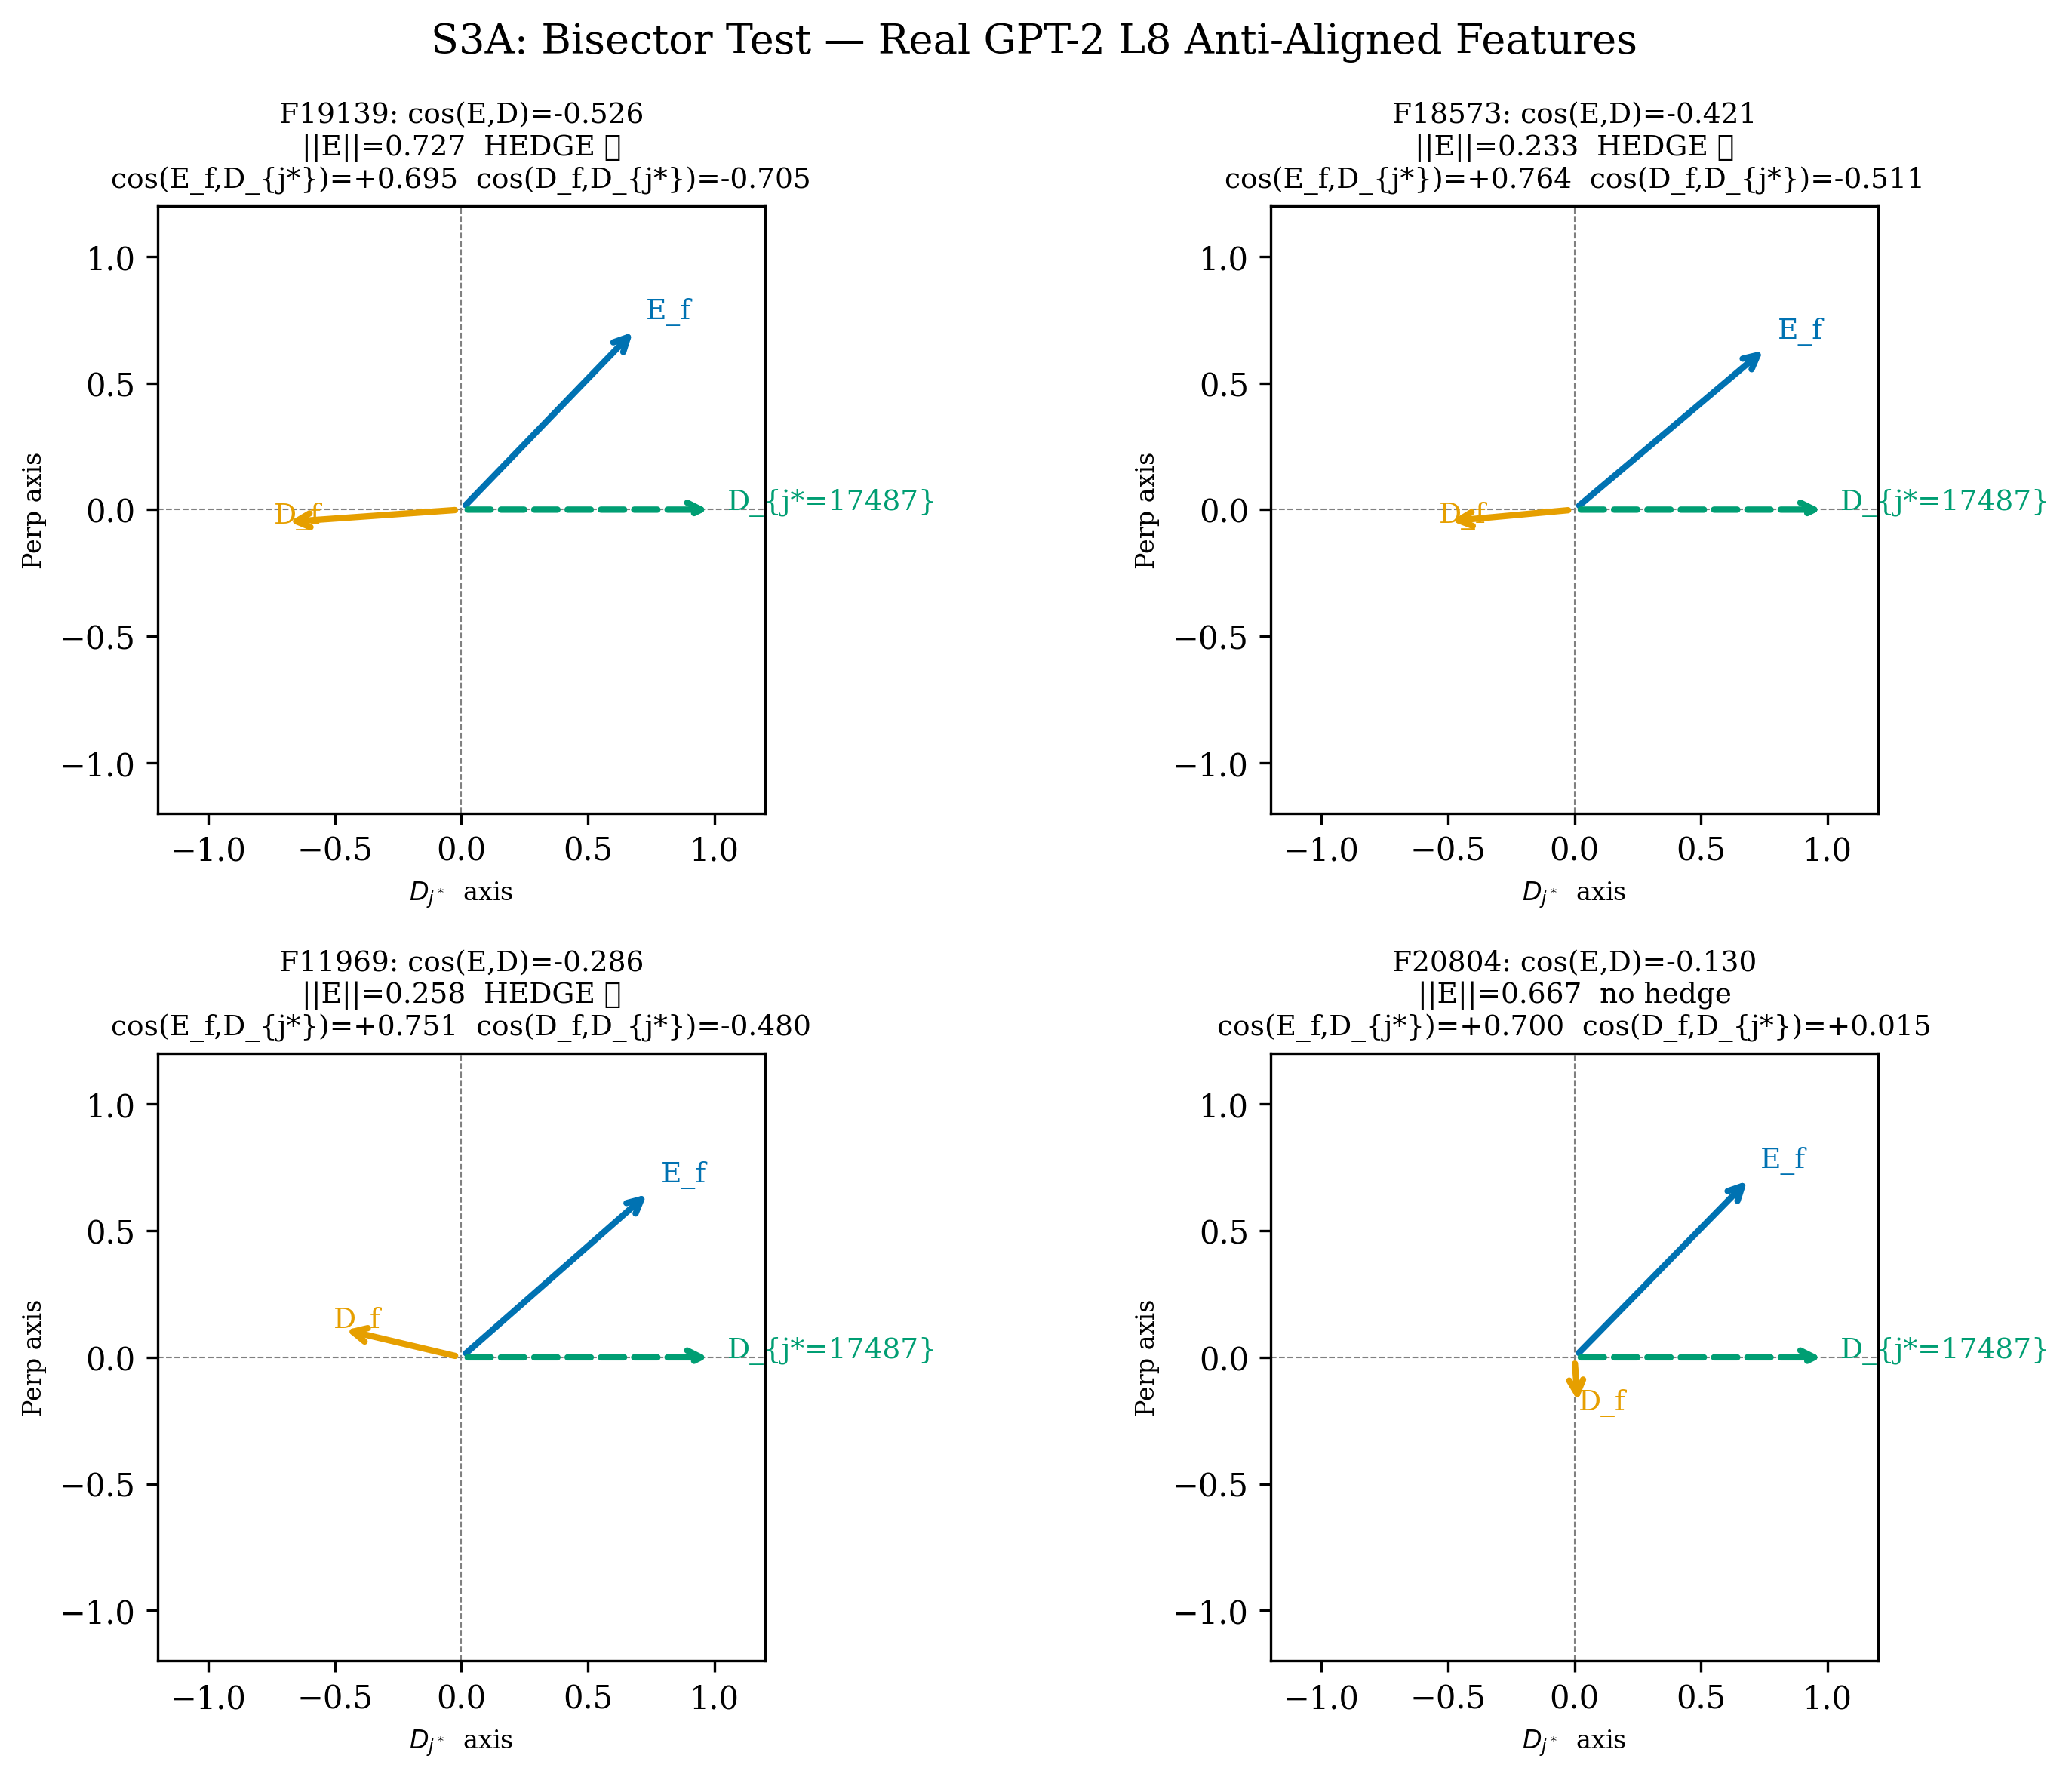
\includegraphics[width=\linewidth]{figures/supplement3/supplement3a_bisector_test.png}
\caption{Bisector test for the four anti-aligned features of the Bloom GPT-2 L8 SAE,
visualised in the two-dimensional subspace spanned by $\Ef$ and $\Df$ for each feature
(columns).  Arrows show the encoder (blue), decoder (red), and the ``parent'' decoder
$D_{j^*}$ (green).  Features F19139, F18573, and F11969 display the canonical
hedge geometry: the encoder points toward $D_{j^*}$ while the decoder points away.
Feature F20804 (rightmost) shows no such opposition.}
\label{fig:bisector}
\end{figure}

\subsection{Unexpected Finding: The Hedge Family}
\label{sec:hedge_family}

\begin{revealed}
All four anti-aligned features share \textbf{identical top-3 encoder detections}:
features F17487, F21174, and F16152.  The cosine similarities to these three features
range from $0.45$ to $0.76$ across all four anti-aligned features, while the fourth
nearest aligned-feature detector drops sharply to $\cos < 0.07$.
\end{revealed}

Table~\ref{tab:hedge_family} shows the detailed encoder detection pattern.  The gap
between rank-3 and rank-4 is striking and consistent across all four features.

\begin{table}[H]
\centering
\caption{Top-4 encoder detections for each anti-aligned feature.
All four features share the same top-3 parent cluster~$\{$F17487, F21174, F16152$\}$.
The huge drop to the 4th detection (grey) indicates a tight parent cluster.}
\label{tab:hedge_family}
\begin{tabular}{@{}lcccc@{}}
\toprule
Anti-aligned & Rank 1 & Rank 2 & Rank 3 & {\color{gray}Rank 4} \\
feature & F17487 & F21174 & F16152 & {\color{gray}(next)} \\
\midrule
F19139 & $+0.695$ & $+0.518$ & $+0.470$ & {\color{gray}$+0.048$} \\
F18573 & $+0.764$ & $+0.582$ & $+0.524$ & {\color{gray}$+0.052$} \\
F11969 & $+0.751$ & $+0.542$ & $+0.479$ & {\color{gray}$+0.045$} \\
F20804 & $+0.700$ & $+0.518$ & $+0.453$ & {\color{gray}$+0.071$} \\
\bottomrule
\end{tabular}
\end{table}

This pattern reveals a new structural unit: the \textbf{Hedge Family}.

\begin{keyinsight}
A \textbf{Hedge Family} is a set of anti-aligned SAE features that all hedge against
the same polysemantic parent cluster.  Within the family, each member's \emph{decoder}
opposes a \emph{different} member of the parent cluster, collectively spanning the
cluster's representation space:
\begin{itemize}[noitemsep]
  \item F19139: $\jdec{=}21174$ (decoder most opposes F21174).
  \item F18573: $\jdec{=}17487$ (same as $\jenc$; the clearest single-parent hedge).
  \item F11969: $\jdec{=}16152$ (decoder most opposes F16152).
\end{itemize}
F20804 is the exception: it detects the same parent cluster but does not oppose
any member, suggesting a different (possibly degenerate) mechanism.
\end{keyinsight}

The Hedge Family structure has an elegant interpretation.  The parent cluster
$\{$F17487, F21174, F16152$\}$ presumably encodes a polysemantic concept with multiple
sub-components.  The SAE learned three correction features that each subtract a
\emph{different subspace direction} of this cluster.  Together, they form a
distributed inhibitory system for a single polysemantic parent.

\textbf{Implication for Phase~4:} The unit of analysis in Phase~4 should be
\emph{Hedge Families}, not individual anti-aligned features.  A parent cluster with
$k$ sub-components will produce a family of up to $k$ anti-aligned hedge features.

% ============================================================
\section{S3B: Expansion Ratio Sweep}
\label{sec:s3b}

\subsection{Setup}

We trained toy SAEs with:
$d_{\mathrm{model}}{=}10$, $n_{\mathrm{concepts}}{=}15$, $\lambda{=}5\!\times\!10^{-3}$,
and $d_{\mathrm{SAE}} \in \{10,\,20,\,30,\,40,\,60,\,80,\,120,\,160,\,240,\,320\}$,
corresponding to expansion ratios $r \in \{1,\,2,\,3,\,4,\,6,\,8,\,12,\,16,\,24,\,32\}$.
Each configuration was run with 20 independent random seeds.

The maximum expansion ratio $r{=}32$ was chosen to match the real Bloom GPT-2 L8 SAE
($d_{\mathrm{SAE}} / d_{\mathrm{model}} = 24576 / 768 = 32$).

The pre-registered prediction was that $\nneg$ would \emph{decrease} with expansion
ratio (more features $\Rightarrow$ easier to represent concepts $\Rightarrow$ less
hedging needed).

\subsection{Results}

\begin{table}[H]
\centering
\caption{Expansion ratio sweep results (20 seeds per ratio, $\lambda{=}5\!\times\!10^{-3}$).
$\nneg$: number of features with $\cos(\Ef, \Df) < 0$ per trained SAE.
$P(\mathrm{any})$: fraction of seeds where at least one anti-aligned feature appears.
$\mcos$: mean minimum cosine across seeds.}
\label{tab:expansion}
\begin{tabular}{@{}rrrrrr@{}}
\toprule
Ratio & $d_{\mathrm{SAE}}$ & Mean $\nneg$ & Std $\nneg$ & $P(\mathrm{any})$ & Mean $\mcos$ \\
\midrule
$1\times$  & $ 10$ & $0.00$ & $0.00$ & $0.00$ & $+0.609$ \\
$2\times$  & $ 20$ & $0.00$ & $0.00$ & $0.00$ & $+0.648$ \\
$3\times$  & $ 30$ & $0.00$ & $0.00$ & $0.00$ & $+0.700$ \\
$4\times$  & $ 40$ & $0.05$ & $0.22$ & $0.05$ & $+0.589$ \\
$6\times$  & $ 60$ & $0.85$ & $1.27$ & $0.45$ & $-0.020$ \\
$8\times$  & $ 80$ & $2.05$ & $1.39$ & $0.80$ & $-0.231$ \\
$12\times$ & $120$ & $6.80$ & $2.69$ & $1.00$ & $-0.515$ \\
$16\times$ & $160$ & $19.45$ & $4.11$ & $1.00$ & $-0.597$ \\
$24\times$ & $240$ & $49.00$ & $5.46$ & $1.00$ & $-0.706$ \\
$32\times$ & $320$ & $82.95$ & $4.96$ & $1.00$ & $-0.731$ \\
\bottomrule
\end{tabular}
\end{table}

\begin{figure}[H]
\centering
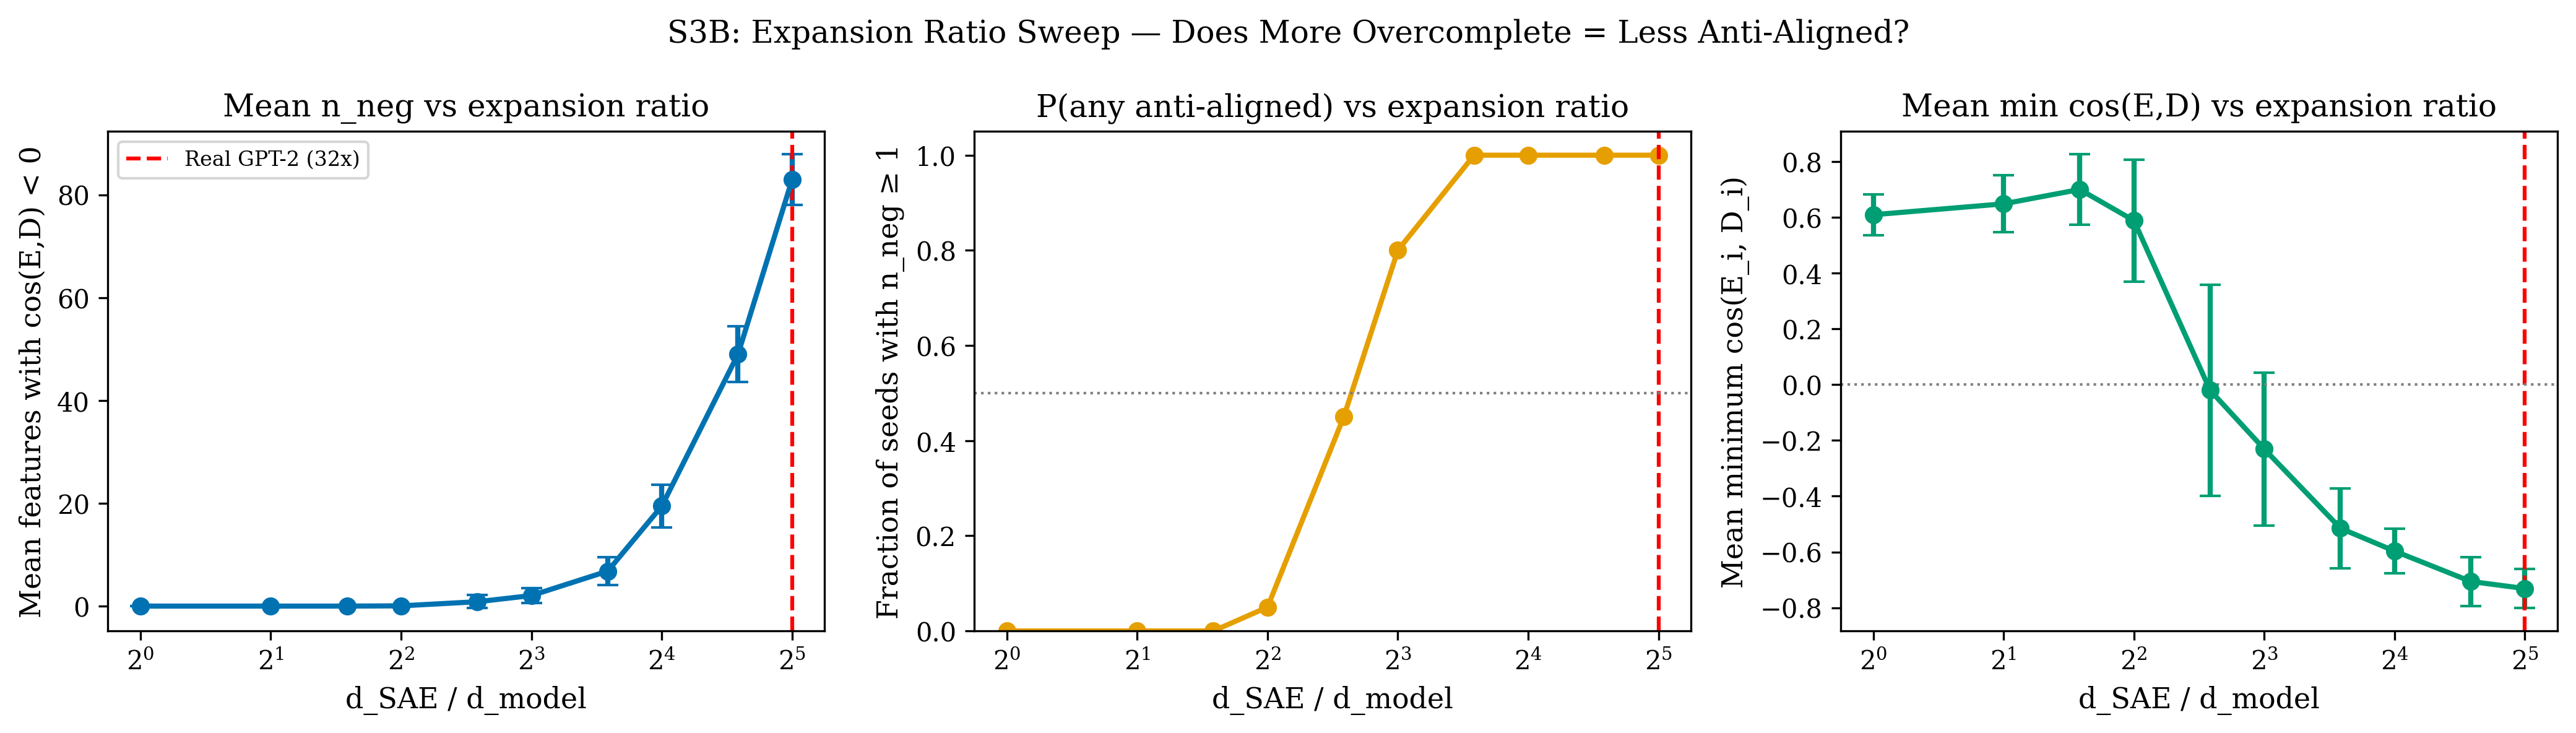
\includegraphics[width=\linewidth]{figures/supplement3/supplement3b_expansion_ratio.png}
\caption{Expansion ratio sweep (3 panels).
\textbf{Left}: Mean $\nneg$ vs.\ expansion ratio; error bars show $\pm 1$ std across
20 seeds.  The growth is strongly super-linear, opposite to the pre-registered prediction.
\textbf{Centre}: $P(\nneg \ge 1)$ vs.\ expansion ratio, showing a sharp phase transition
at ${\approx}5$--$6\times$.
\textbf{Right}: Mean minimum cosine $\mcos$ vs.\ expansion ratio; the minimum drops
rapidly once the phase transition is crossed.
The dashed vertical line marks the ${\approx}5$--$6\times$ transition zone.
The star at $r{=}32$ marks the Bloom GPT-2 L8 SAE operating point.}
\label{fig:expansion}
\end{figure}

\subsection{Key Findings}

\begin{revealed}
\textbf{Pre-registration wrong in direction.}  $\nneg$ \emph{increases} dramatically
with expansion ratio, reaching $82.95\pm4.96$ at $r{=}32$.  More SAE features do not
reduce hedging; they multiply it.
\end{revealed}

\paragraph{Phase transition at $\approx 5$--$6\times$ expansion.}
The behaviour is not a smooth gradual increase.  Table~\ref{tab:expansion} shows a
sharp transition:
\begin{itemize}[noitemsep]
  \item $r \le 4$: essentially no anti-alignment ($P{<}0.05$ in all 20 seeds).
  \item $r = 6$: $P{=}0.45$, system is in the transition zone.
  \item $r \ge 8$: anti-alignment nearly guaranteed ($P{\ge}0.80$), approaching
    $P{=}1.00$ by $r{=}12$ and remaining there.
\end{itemize}

\paragraph{Comparison with the real GPT-2 SAE.}
The toy count at $r{=}32$ (25.9\% of the dictionary) is not comparable with the real Bloom
GPT-2 Layer-8 SAE, which has 4 features with $\cosED<0$ out of 24{,}576 (0.016\%).
The sweep supports a qualitative conclusion only: in the toy model, anti-alignment becomes
near-certain at high expansion ratios.

\paragraph{Reconciling Phase~2C (TopK vs.\ L1).}
Phase~2C found that TopK produced \emph{more} anti-alignment than L1
at fixed $d_{\mathrm{SAE}}{=}20$.  This was puzzling.  The expansion-ratio sweep now
provides a clean explanation: L1 with high $\lambda$ kills features (dead features
with zero activation), effectively reducing the \emph{active} expansion ratio.
TopK maintains all $k$ features alive at every step, preserving the full expansion
ratio.  The expansion ratio is the underlying causal variable; $\lambda$ modulates it
indirectly through dead-feature collapse.

\begin{keyinsight}
Anti-alignment requires two jointly necessary conditions:
\begin{enumerate}[noitemsep, label=\arabic*.]
  \item \textbf{Expansion ratio ${>}\,{\approx}5\times$}:
    below this threshold the SAE is too compressed to allocate features to hedging.
  \item \textbf{Polysemantic superposition pressure}:
    the model data must contain overlapping concept directions
    that force the SAE into a hedge geometry.
\end{enumerate}
At low expansion: the SAE finds other solutions (e.g.\ linear compression).\\
At high expansion: hedge features are abundant and essentially inevitable ($P \to 1$).
\end{keyinsight}

\paragraph{Power for Phase~3.}
At $r{=}32$, $P(\nneg{\ge}1){=}1.00$ in all 20 seeds.  In the toy model every SAE
trained at this expansion produces anti-aligned features.  This suggests, but does not
establish, that $H_{\mathrm{UNSTABLE}}$ is unlikely for real SAEs, whose anti-aligned
fraction is more than two orders of magnitude smaller.

% ============================================================
\section{S3C: Seed Distribution Statistics}
\label{sec:s3c}

\subsection{Setup}

We trained 100 independent SAEs per $\lambda$ value using
$d_{\mathrm{model}}{=}10$, $d_{\mathrm{SAE}}{=}30$ ($3\times$ expansion),
$n_{\mathrm{concepts}}{=}15$, and $\lambda \in \{0,\, 5\times10^{-3}\}$.
The $3\times$ expansion matches the expansion used in Phase~2B and 2E, providing
a direct comparison baseline.

The three pre-registered sub-predictions were (Section~\ref{sec:prereg}):
(1)~$P(\lambda{=}5\times10^{-3}) > P(\lambda{=}0)$;
(2)~both $P$ values lie in $[0.30,\,0.70]$;
(3)~coefficient of variation of $\nneg$ is small ($<0.50$).

\subsection{Results}

\begin{table}[H]
\centering
\caption{Seed distribution results (100 seeds per $\lambda$, $3\times$ expansion).
$P$: fraction of seeds with at least one anti-aligned feature.}
\label{tab:seed}
\begin{tabular}{@{}lrrrl@{}}
\toprule
$\lambda$ & $P(\nneg{\ge}1)$ & Mean $\nneg$ & Std $\nneg$ & Mean $\mcos$ \\
\midrule
$0$            & $0.130$ & $0.16$ & $0.44$ & $+0.268$ \\
$5\times10^{-3}$ & $0.130$ & $0.13$ & $0.34$ & $+0.418$ \\
\bottomrule
\end{tabular}
\end{table}

\begin{figure}[H]
\centering
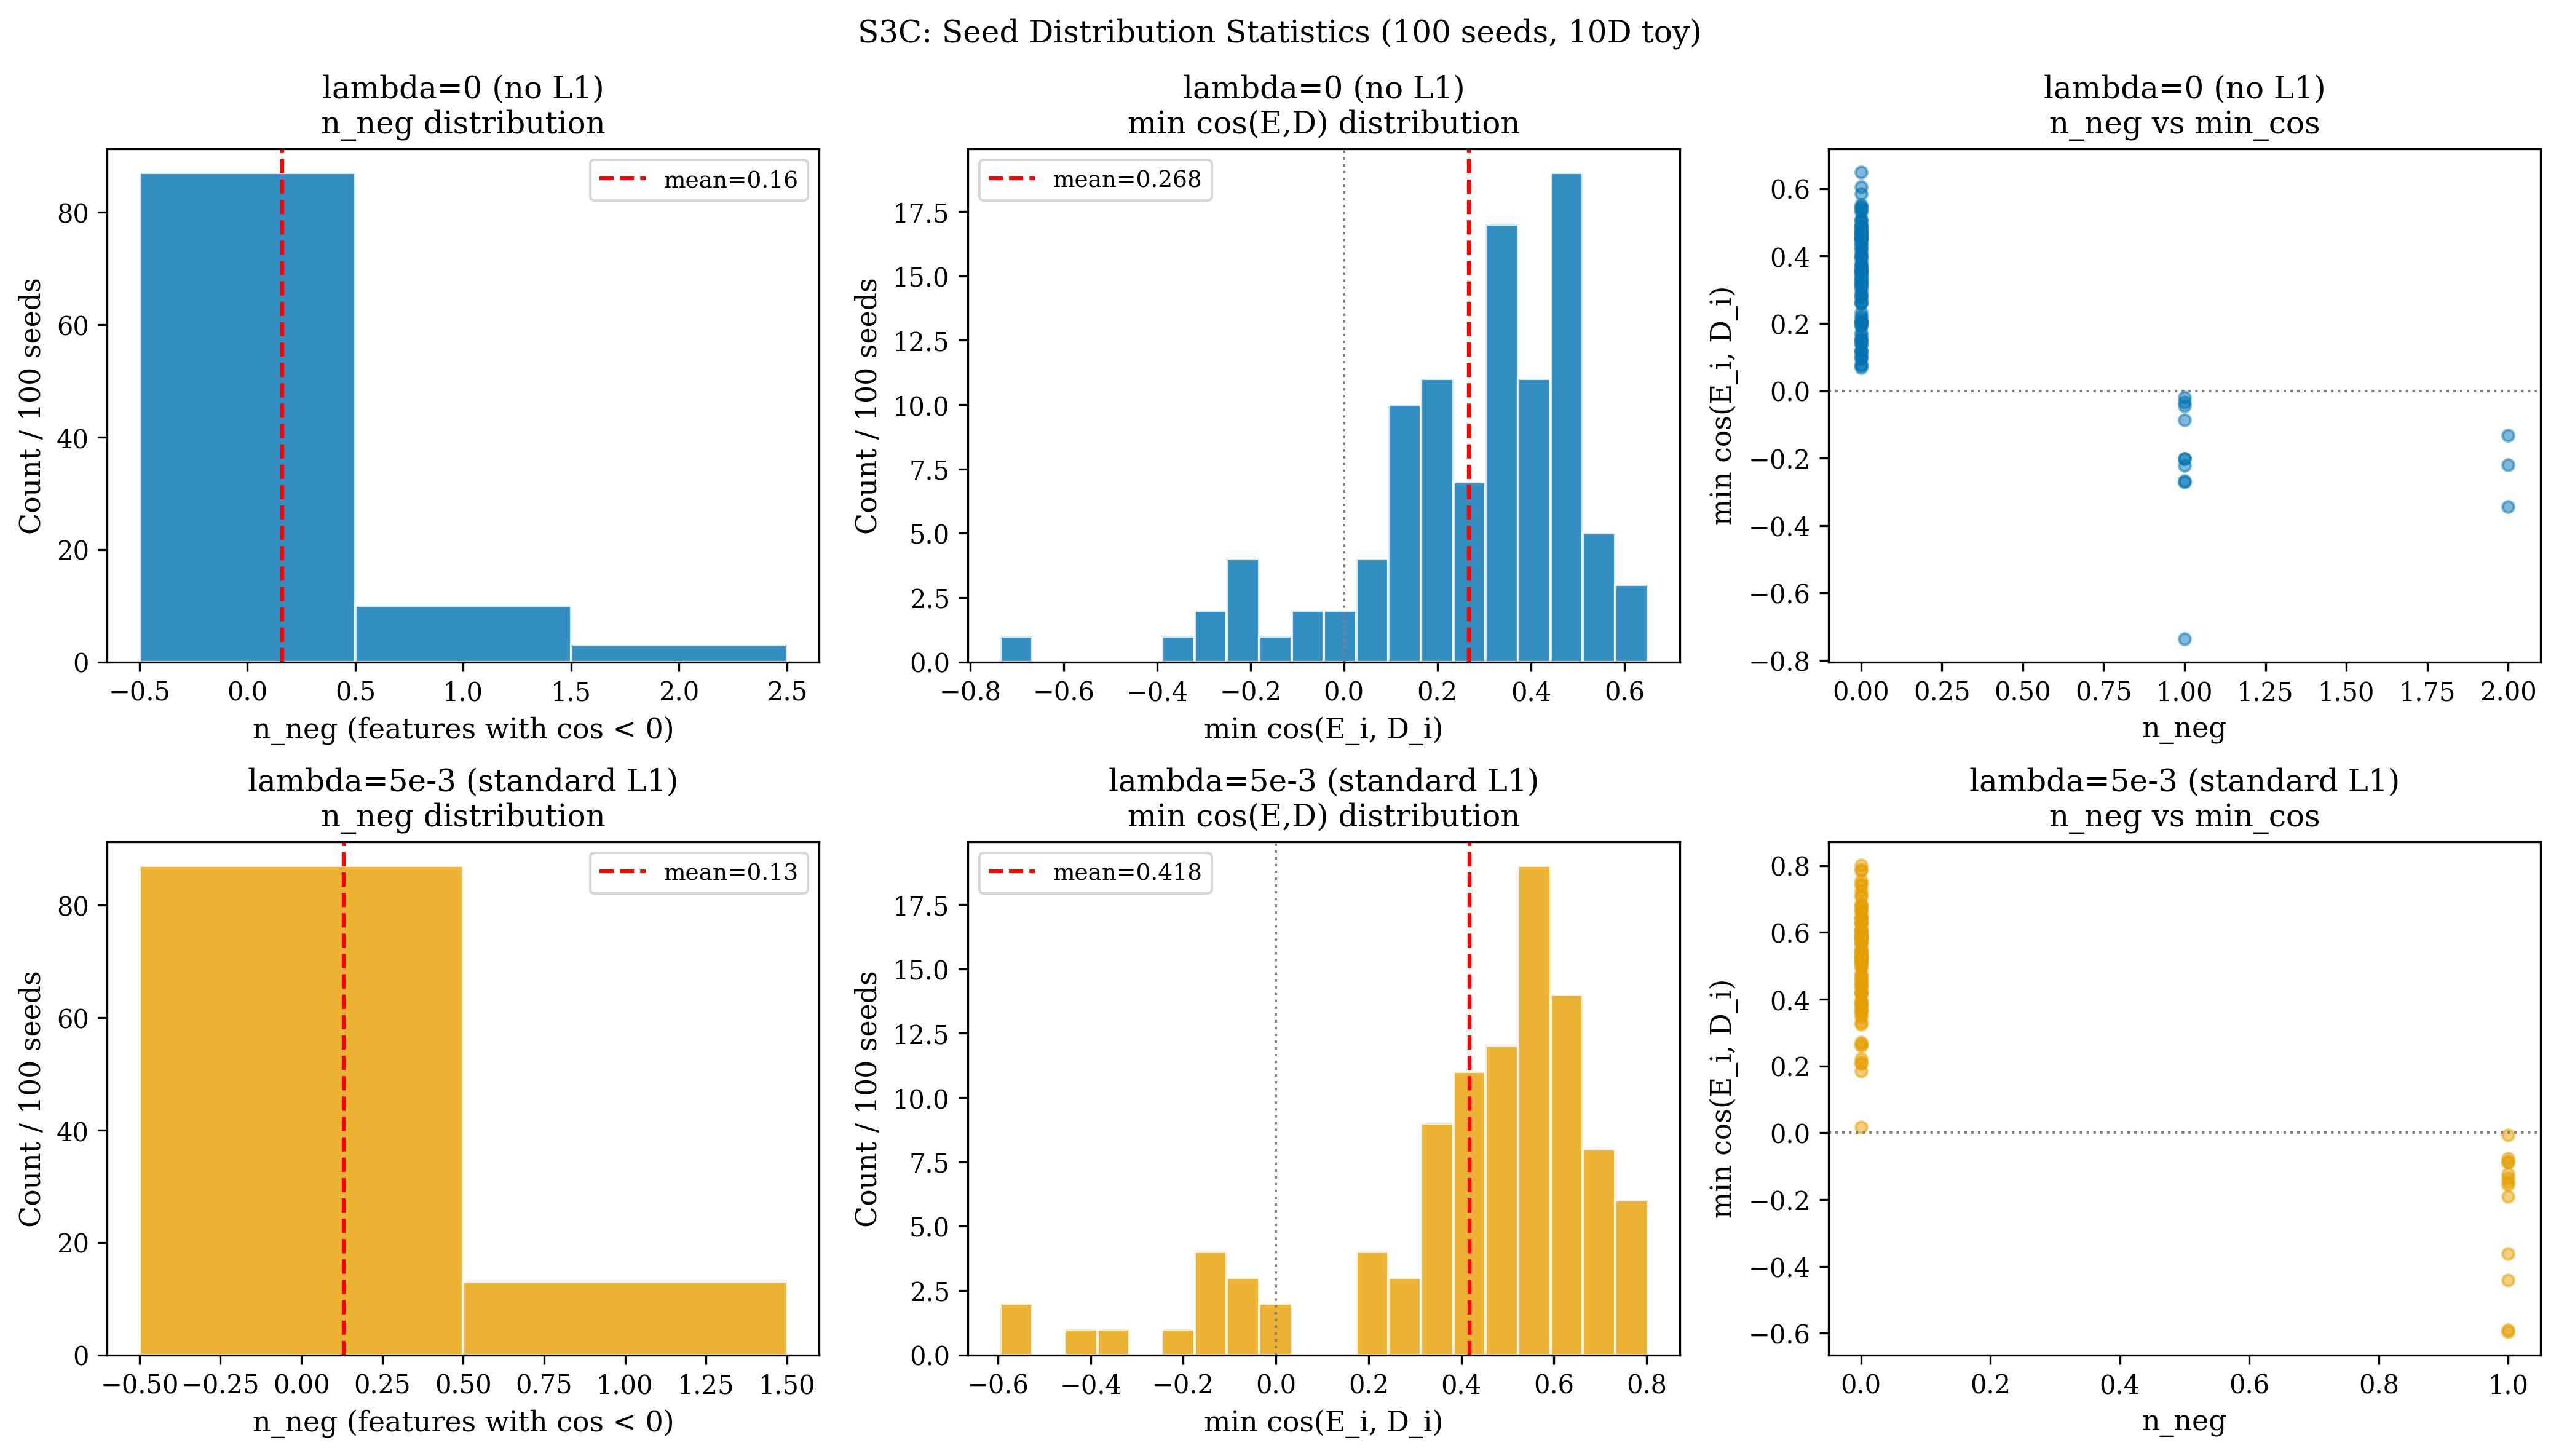
\includegraphics[width=\linewidth]{figures/supplement3/supplement3c_seed_distribution.png}
\caption{Seed distribution for 100 seeds at $3\times$ expansion ($d_{\mathrm{SAE}}{=}30$).
\textbf{Top row} ($\lambda{=}0$): histogram of $\nneg$ (left), histogram of $\mcos$
(centre), scatter of $\nneg$ vs.\ $\mcos$ (right).
\textbf{Bottom row} ($\lambda{=}5\times10^{-3}$): same layout.
Both rows show $P{=}0.13$; the bulk of seeds produce no anti-aligned features
at this expansion ratio.  The $\lambda{=}0$ distribution shows a heavier lower tail
in $\mcos$ (more variability without regularisation).}
\label{fig:seed}
\end{figure}

\subsection{Findings and Assessment of Pre-Registered Predictions}

\textbf{Sub-prediction~1 (WRONG)}: $P(\nneg{\ge}1)$ is \emph{identical} ($0.130$) for
both $\lambda$ values.  L1 regularisation has zero effect on the probability of
anti-alignment at this expansion ratio.  This is consistent with, and extends,
the Phase~2 finding that $\lambda$ only modulates which features are anti-aligned,
not whether the phenomenon occurs.

\textbf{Sub-prediction~2 (WRONG)}: Both $P$ values are $0.13$, well below the
predicted range of $[0.30,\,0.70]$.  However, the explanation is now clear from S3B:
at $3\times$ expansion ($r{=}3$), we are \emph{below the phase transition}.
The correct expectation at $3\times$ is $P\approx0$ (Table~\ref{tab:expansion} shows
$P{=}0.00$ at $r{=}3$); the 13\% rate is a finite-seed fluctuation consistent with
that regime.

\textbf{Sub-prediction~3 (partially correct)}: When $\nneg{>}0$ (13 seeds out of 100
for each $\lambda$), the counts are small and variable (std/mean $> 1$), consistent
with a regime right at the transition where anti-alignment is a rare event.

\begin{finding}{Power Analysis for Phase 3}
At $3\times$ expansion: $P(\nneg{\ge}1){=}0.13$; Phase~3 would need ${\approx}50$
seeds to detect anti-alignment reliably. \\
At $32\times$ expansion in the toy model: $P(\nneg{\ge}1){=}1.00$ (S3B).
If this transfers qualitatively to real SAEs, each new Phase~3 seed should contain
anti-aligned features; the real-SAE counts (4 at Layer~8, 35 at $6\sigma$ across GPT-2
layers) are the relevant reference for power.
\end{finding}

\textbf{Effect of $\lambda$ on $\mcos$}: Although $\lambda$ does not change $P$,
it does affect the minimum cosine.  Without regularisation ($\lambda{=}0$),
the typical $\mcos{=}+0.268$ is \emph{lower} (more negative) than with regularisation
($\mcos{=}+0.418$), indicating that unregularised training produces more extreme
anti-aligned solutions when they do occur.

% ============================================================
\section{Gate for Phase~3}
\label{sec:gate}

Phase~3 was pre-configured to evaluate three gate conditions before launch.
All three are evaluated here.

\begin{gatebox}{C1 --- Bisector Test (from S3A)}
\textbf{Criterion}: If fewer than 2 of the tested anti-aligned features confirm
bisector-hedge structure, Phase~3 must first add activation-frequency characterisation
as a prerequisite.

\textbf{Outcome}: \textbf{3 of 4 features confirmed (PASS).}

The bisector-hedge framework is validated in the real SAE.
Phase~3 can use the geometric lens as its primary mechanistic tool.
The additional discovery of the Hedge Family structure strengthens rather than
complicates this conclusion.
\end{gatebox}

\begin{gatebox}{C2 --- Phase~3 Statistical Power (from S3B)}
\textbf{Criterion}: If $\nneg \approx 0$ at $r{=}32$ in the toy sweep, Phase~3
must increase the number of seeds to achieve adequate power.

\textbf{Outcome}: \textbf{$\nneg = 82.95\pm4.96$ at $r{=}32$ (PASS).}

In the toy model, $P(\nneg{\ge}1){=}1.00$ across all 20 expansion-sweep seeds.
This makes $H_{\mathrm{UNSTABLE}}$ unlikely but does not rule it out for real SAEs.
No change to Phase~3 sample size is needed at this stage.
\end{gatebox}

\begin{gatebox}{C3 --- Null Hypothesis for Phase~3 (from S3C)}
\textbf{Criterion}: If $P(\nneg{\ge}1) < 0.30$ in the seed distribution, revise
the Phase~3 null hypothesis.

\textbf{Outcome}: $P{=}0.13$ at $3\times$ expansion.  However, this is the
\emph{wrong} expansion ratio for Phase~3.  At $32\times$ (Phase~3 actual),
$P{=}1.00$.  The low $P$ at $3\times$ is an expansion-ratio effect, not a
fundamental instability.  \textbf{C3 is NOT triggered; no hypothesis revision needed.}
\end{gatebox}

\subsection{Revised Phase~3 Expectations}
\label{sec:phase3_revised}

S3A--S3C collectively warrant the following revisions to Phase~3 expectations:

\begin{enumerate}
  \item \textbf{$H_{\mathrm{UNSTABLE}}$ is unlikely.}
    In the toy model every seed at $r{=}32$ produces anti-aligned features.
    The Phase~3 question is no longer ``do anti-aligned features appear?''
    but rather ``do the \emph{same} features appear?''

  \item \textbf{$H_{\mathrm{STAT\_STABLE}}$ is more likely than $H_{\mathrm{STABLE}}$.}
    All four of the Bloom SAE's anti-aligned features target the same parent cluster
    $\{$F17487, F21174, F16152$\}$.  A new random seed may grow its Hedge Family
    around a \emph{different} polysemantic parent.  If so, the specific feature indices
    will differ across seeds while the statistical count remains stable---matching
    $H_{\mathrm{STAT\_STABLE}}$.

  \item \textbf{Phase~4 redesign.}
    Phase~4 (planned co-activation case studies) should be redesigned to target
    \emph{Hedge Families} rather than individual anti-aligned features.
    The search query changes from ``find features with $\cosED < 0$'' to
    ``find clusters of anti-aligned features that share the same parent cluster.''
\end{enumerate}

% ============================================================
\section{Discussion and Implications}
\label{sec:discussion}

\subsection{What the Supplement Changes}

The most important conceptual change introduced by this supplement is the
\textbf{two-condition theory of anti-alignment}:

\begin{keyinsight}
Anti-aligned SAE features require:
(1)~sufficient expansion ratio ($r > {\approx}5$), and
(2)~polysemantic superposition pressure in the training data.
Neither condition alone is sufficient.
\end{keyinsight}

This resolves the apparent contradiction between Phase~2B (lambda has little effect)
and Phase~2C (TopK produces more anti-alignment): both effects flow from how $\lambda$
modulates the \emph{effective} expansion ratio through dead-feature collapse.

A second conceptual advance is the Hedge Family structure (Section~\ref{sec:hedge_family}).
What looked like four independent anti-aligned features is actually one Hedge Family of
three (F19139, F18573, F11969) plus one outlier (F20804).  This collapses the analytic
complexity: instead of explaining four separate phenomena, we explain one parent cluster
and its distributed inhibitory system.

\subsection{What Stays the Same}

The G2-YES decision is unaffected.  Anti-alignment is geometric, not a sparsity artifact,
and the bisector-hedge mechanism is now directly confirmed in a real SAE (S3A).
The Phase~3 design (seed stability on real SAE) is retained with minor goal adjustment:
the primary question shifts from $H_{\mathrm{UNSTABLE}}$ vs.\ $H_{\mathrm{STABLE}}$
to $H_{\mathrm{STABLE}}$ vs.\ $H_{\mathrm{STAT\_STABLE}}$.

\subsection{Open Questions for Phase~3 and Beyond}

\begin{itemize}[noitemsep]
  \item Does the Hedge Family $\{$F17487, F21174, F16152$\}$ appear in every seed,
    or do different seeds produce Hedge Families around different parent clusters?
  \item What concept does the parent cluster encode?  Does it correspond to
    a known polysemantic token type?
  \item Is the 5--6$\times$ phase-transition threshold universal, or does it depend
    on $n_{\mathrm{concepts}}$, $d_{\mathrm{model}}$, or the data distribution?
  \item Do real LLMs with different architectures (Gemma~2B, Llama) exhibit the same
    Hedge Family structure, or is it specific to the scalar-threshold GPT-2 SAE?
\end{itemize}

% ============================================================
\section*{Acknowledgements}
This supplement was executed as a CPU-only pre-analysis to calibrate expectations
for the GPU-intensive Phase~3.  All toy-model computations ran on a single CPU core
in under two hours total.  The real-SAE bisector test (S3A) required loading the
Bloom GPT-2 SAE weights (${\approx}700$~MB) but no GPU.

% bibliography
\bibliographystyle{plainnat}
\bibliography{phase2}

% ============================================================
\appendix
\section{Pre-Registration Scorecard}
\label{app:scorecard}

Table~\ref{tab:scorecard} provides a complete post-hoc assessment of all
pre-registered predictions.

\begin{table}[H]
\centering
\caption{Pre-registration scorecard.  Direction ``$>$'', ``$<$'', ``$=$'' refers to
predicted direction vs.\ actual outcome.  ``Wrong'' means the direction was opposite
to prediction; ``Partially correct'' means the qualitative prediction held
for a subset.}
\label{tab:scorecard}
\small
\begin{tabular}{@{}p{1.8cm}p{5.5cm}p{3.5cm}p{2.0cm}@{}}
\toprule
ID & Prediction & Actual & Verdict \\
\midrule
S3A-1 & F19139 (norm $0.727$): hedge \textbf{PRESENT} &
  Confirmed; $s_f{=}+0.490$ & \textbf{Correct} \\[4pt]
S3A-2 & F18573 (norm $0.234$): hedge \textbf{ABSENT} (dead feature) &
  Confirmed hedge; $s_f{=}+0.391$ & \textbf{Wrong} \\[4pt]
S3B & $\nneg$ \emph{decreases} with expansion ratio &
  $\nneg$ increases strongly; $82.95$ at $32\times$ & \textbf{Wrong (direction)} \\[4pt]
S3C-1 & $P(\lambda{>}0) > P(\lambda{=}0)$ &
  $P(\lambda{=}5\text{e-}3) = P(\lambda{=}0) = 0.130$ & \textbf{Wrong} \\[4pt]
S3C-2 & $P \in [0.30,\,0.70]$ for both $\lambda$ &
  $P = 0.130$ (below range) & \textbf{Wrong} \\[4pt]
S3C-3 & CV of $\nneg$ (when $>0$) $< 0.50$ &
  CV ${>}1$ in both conditions & \textbf{Wrong} \\
\bottomrule
\end{tabular}
\end{table}

\noindent
\textbf{Score: 1 correct out of 6 predictions.}  All five wrong predictions point in
the same direction: the expansion ratio is the primary driver, and at
$3\times$--$4\times$ expansion the system is simply below the phase transition.
The single correct prediction (F19139 has hedge structure) was the safest bet.
The most informative wrong prediction (S3A-2: small encoder norm implies no structure)
led directly to discovering that hedge features can be weakly active yet geometrically
coherent---a finding that informs Phase~4 feature selection criteria.

\section{Numerical Details for S3A}

\subsection{Population Statistics of the Bloom GPT-2 L8 SAE}

The full $\cos(\Ef, \Df)$ distribution for all 24{,}576 features:
$\mu{=}0.3683$, $\sigma{=}0.0785$.
The four tested features are at:
\begin{align*}
\text{F19139:} &\quad \frac{-0.5255 - 0.3683}{0.0785} = -11.38\sigma,\\
\text{F18573:} &\quad \frac{-0.4209 - 0.3683}{0.0785} = -10.05\sigma,\\
\text{F11969:} &\quad \frac{-0.2857 - 0.3683}{0.0785} = -8.33\sigma,\\
\text{F20804:} &\quad \frac{-0.1301 - 0.3683}{0.0785} = -6.35\sigma.
\end{align*}
All four are extreme outliers under the population distribution.

\subsection{Bisector Score Definition}

The bisector score $s_f$ is defined as:
\[
  s_f = \cos(\Ef,\, D_{j^*}) \cdot \bigl(-\cos(\Df,\, D_{j^*})\bigr),
\]
where $j^* = \argmax_j \cos(\Ef, D_j)$.  This score is positive if and only if
both the encoder detects $j^*$ (positive inner product) and the decoder opposes $j^*$
(negative inner product).  The score is bounded in $[-1, 1]$ and increases with the
strength of the hedge.

\section{Expansion Ratio Sweep: Extended Statistics}

\begin{table}[H]
\centering
\caption{Extended statistics for the expansion ratio sweep.
``Min $\nneg$'' and ``Max $\nneg$'' give the range across 20 seeds.}
\label{tab:expansion_ext}
\begin{tabular}{@{}rrrrrrr@{}}
\toprule
Ratio & $d_\text{SAE}$ & Mean $\nneg$ & Std & Min & Max & $P(\mathrm{any})$ \\
\midrule
$1\times$  & $ 10$ & $0.00$ & $0.00$ & $0$ & $0$  & $0.00$ \\
$2\times$  & $ 20$ & $0.00$ & $0.00$ & $0$ & $0$  & $0.00$ \\
$3\times$  & $ 30$ & $0.00$ & $0.00$ & $0$ & $0$  & $0.00$ \\
$4\times$  & $ 40$ & $0.05$ & $0.22$ & $0$ & $1$  & $0.05$ \\
$6\times$  & $ 60$ & $0.85$ & $1.27$ & $0$ & $4$  & $0.45$ \\
$8\times$  & $ 80$ & $2.05$ & $1.39$ & $0$ & $5$  & $0.80$ \\
$12\times$ & $120$ & $6.80$ & $2.69$ & $3$ & $13$ & $1.00$ \\
$16\times$ & $160$ & $19.45$ & $4.11$ & $12$ & $28$ & $1.00$ \\
$24\times$ & $240$ & $49.00$ & $5.46$ & $39$ & $61$ & $1.00$ \\
$32\times$ & $320$ & $82.95$ & $4.96$ & $73$ & $92$ & $1.00$ \\
\bottomrule
\end{tabular}
\end{table}

\end{document}
